\section{Introdução} \bigskip
Nos dias de hoje, o voluntariado é cada vez mais praticado na nossa sociedade. Segundo um estudo realizado pelo INE - Instituto Nacional de Estatística, em 2019, cerca de 6,4\% da população portuguesa realiza trabalho voluntário, uma percentagem que cresceu ligeiramente face aos resultados obtidos em 2012 (5,9\%).~\cite{estatistica_2019}
\par \bigskip

O trabalho voluntário, ou voluntariado, segundo o diário da república, tem como definição: \par \bigskip

\textit{
	``O conjunto de ações de interesse social e comunitário realizadas de forma desinteressada por pessoas, no âmbito de projetos, programas e outras formas de intervenção ao serviço dos indivíduos, das famílias e da comunidade desenvolvidos sem fins lucrativos por entidades públicas ou privadas.''~\cite{decreto_lei_71/98}
}\par \bigskip

Cabe assim ao voluntário (pessoa que realiza o voluntariado) e entidades o papel fulcral na sociedade de tentar enriquecer a mesma sem qualquer contrapartida. \par \bigskip

Para os voluntários, a participação em ações de voluntariado permite a obtenção de competências multi-disciplinares que são valorizadas no mundo profissional, e como tal, cada vez mais empresas dão valor a candidatos que participam nestas ações. \par \bigskip

Atualmente, a candidatura ao voluntariado é efetuada através de múltiplas plataformas, como redes sociais e \textit{websites}, algo que descentraliza estes serviços porque cada organização usa o seu próprio modelo (figura 1).

\bigskip

\begin{figure}[h]
	\centering
	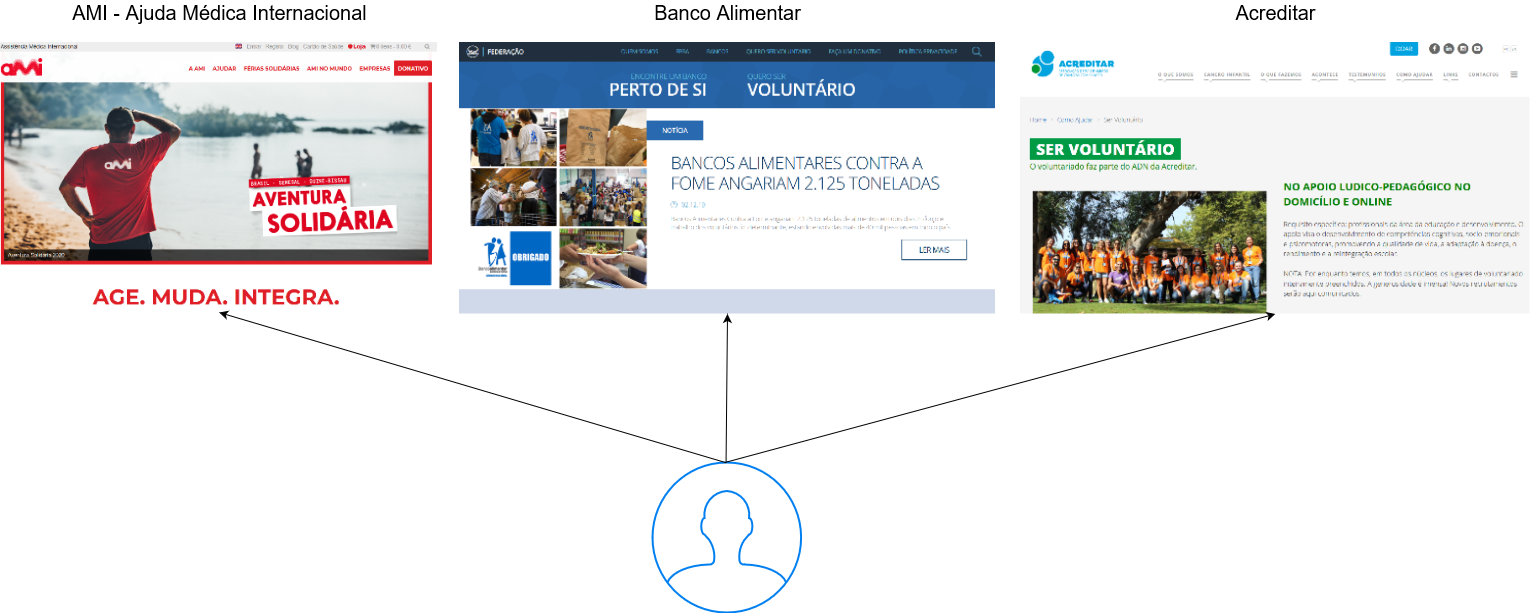
\includegraphics[scale=0.1950]{services-decentralized}
	\caption{Modelo descentralizado de divulgação de voluntariado}	
\end{figure}

\newpage

O nosso projeto tem como objetivo desenvolver uma rede social  com foco no voluntariado. A plataforma proposta irá disponibilizar às entidades organizadoras a possibilidade de divulgar e organizar estas ações, e aos voluntários, serviços que facilitam aos mesmos manterem-se informados e participarem nas ações do seu interesse (figura 2).

\bigskip \bigskip \bigskip

\begin{figure}[h]
	\centering
	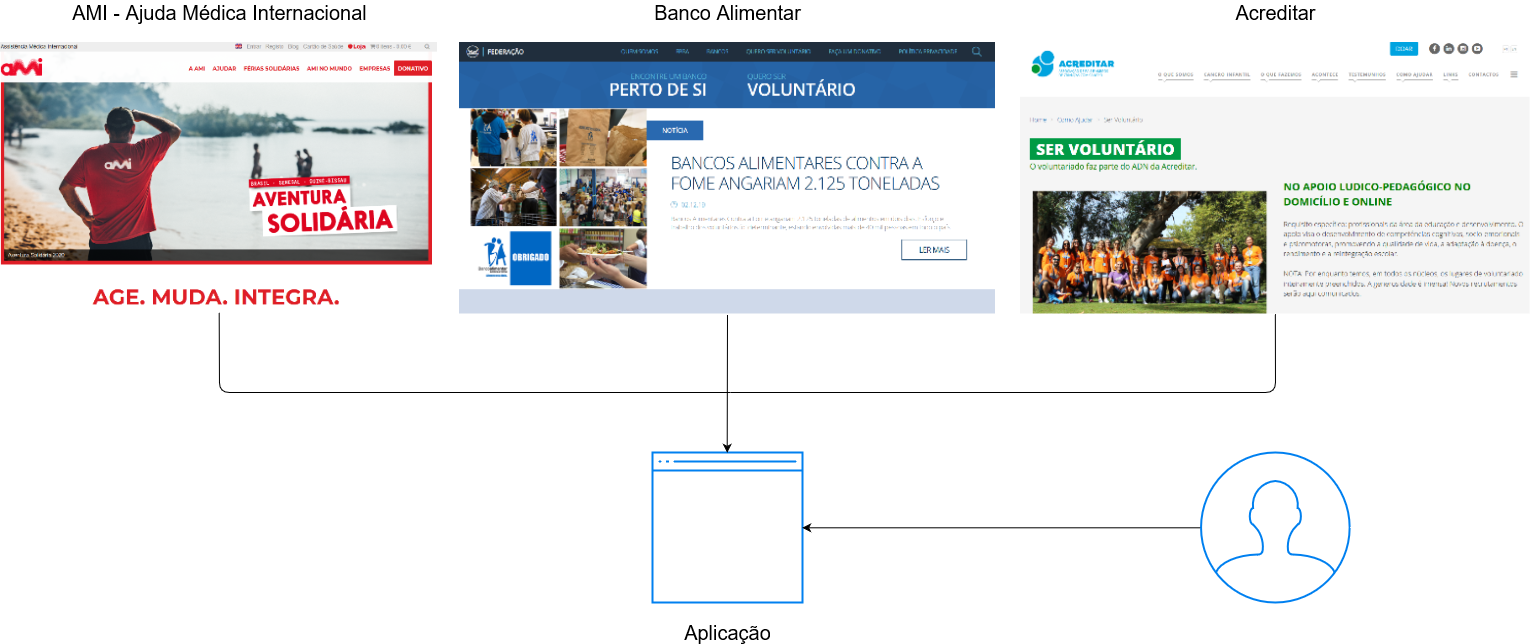
\includegraphics[scale=0.225]{services-centralized}
	\caption{Conceito do projeto}
\end{figure}

\subsection{Organização do relatório}

O presente documento encontra-se organizado em 8 capítulos, descritos de seguida.
\begin{enumerate}
	\item Introdução, onde é realizada a contextualização do projeto e definição da estrutura do relatório do mesmo;
	\item Formulação do problema, onde se faz uma abordagem relativamente a plataformas similares ao projeto desenvolvido, levantando as suas desvantagens. Neste capítulo, são também definidos os requisitos funcionais do projeto;
	\item Modelo de arquitetura, capítulo responsável por discutir a arquitetura geral da plataforma e apresentar os seus módulos principais e as tecnologias utilizadas no desenvolvimento da mesma;
	\item API, onde é descrito o funcionamento da API;
	\item Mobile App, onde se aborda a implementação da aplicação cliente orientada ao voluntário;
	\item Web App, onde se apresenta detalhes relativos ao funcionamento da aplicação cliente orientada à organização;
	\item Planeamento e desenvolvimento do projeto, capítulo que realiza uma comparação entre a calendarização apresentada na proposta de projeto e a calendarização real do mesmo;
	\item Conclusão, onde são apresentadas as conclusões tiradas após o desenvolvimento do projeto.
\end{enumerate}
























